%\newpage
% -----------------------------------------------------------------------
\chapter{Course project}
%-----------------------------------------------------------------------
\section{Raspberry Pi}
Raspberry Pi is a series of small single-board computers developed in the
United Kingdom by the Raspberry Pi Foundation in association with Broadcom.
Early on, the Raspberry Pi project leaned towards the promotion of teaching
basic computer science in schools and in developing countries.
Later, the original model became far more popular than anticipated,
selling outside its target market for uses such as robotics. It is now
widely used in many areas, such as for weather monitoring,
because of its low cost and high portability.

\begin{centering}
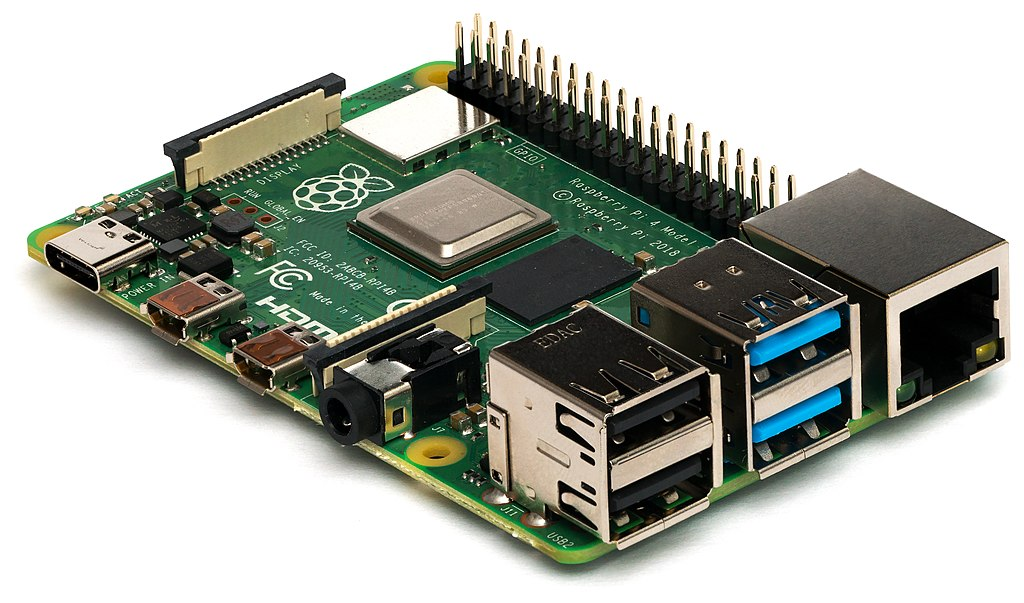
\includegraphics[width=300pt]{images/coursework/raspberrypi.jpeg}\\
(Source: https://www.wikipedia.org)
\end{centering}

\subsection{GPIO}
A powerful feature of the Raspberry Pi is the row of GPIO
(general-purpose input/output) pins along the top edge of the board.
A 40-pin GPIO header is found on all current Raspberry Pi boards.
Any of the GPIO pins can be designated (in software) as an input or output
pin and used for a wide range of purposes.

\begin{centering}
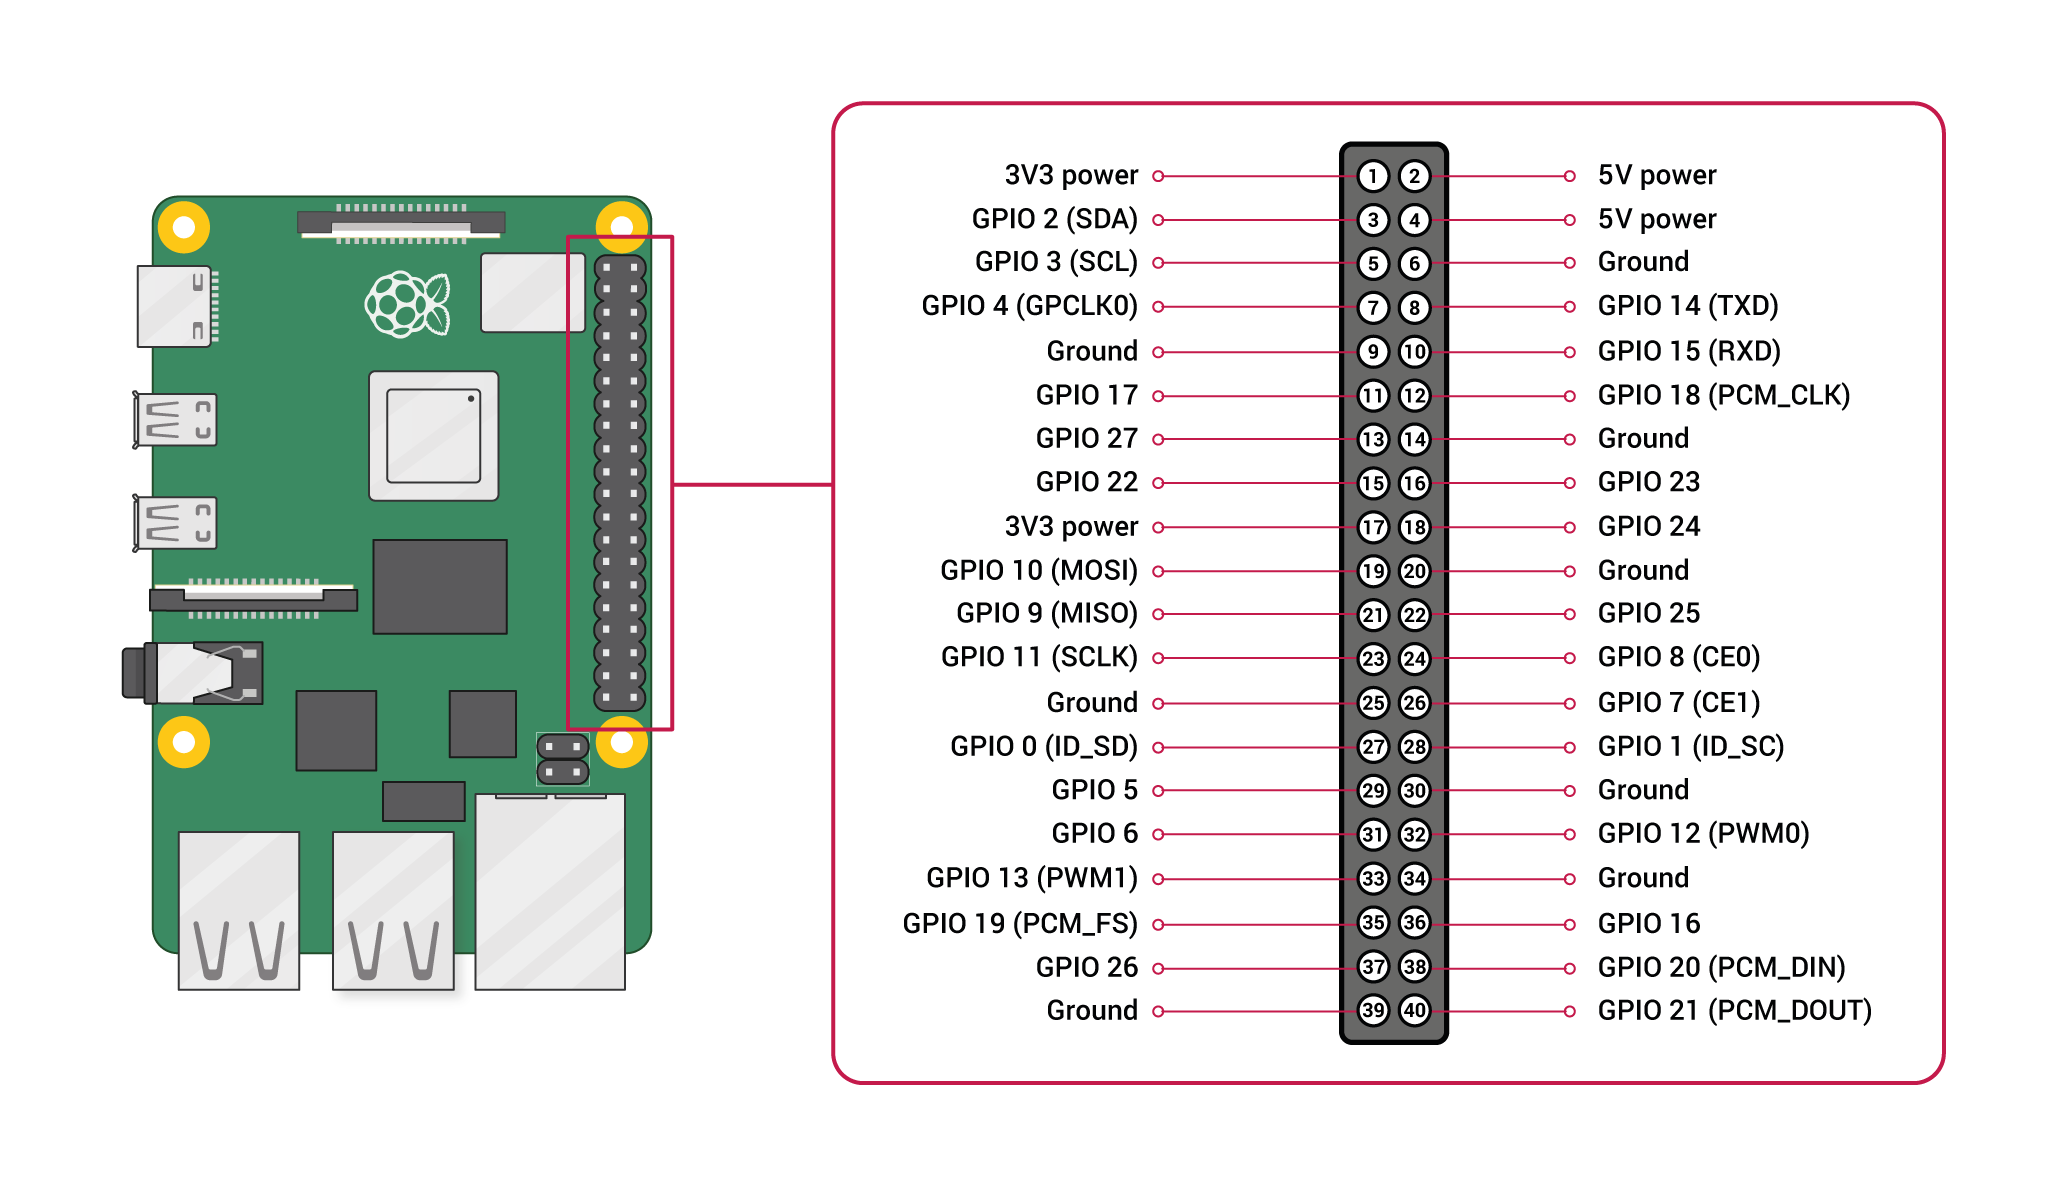
\includegraphics[width=360pt]{images/coursework/gpio.png}\\
(Source: https://www.raspberrypi.org)
\end{centering}

\section{Software}
This software project will develop a web application which could
be used to control external devices which are connected to the
GPIO system of a Raspberry Pi.
